% ======================================================================
\section{Guarantees or compensation}\label{sec:comp}
% ======================================================================

\Cref{sec:sq} protects each person with a floor of their own. The other way to protect people is to pay them. This section sets up compensation as an institution of the same kind, with its own planner and its own guarantee, so that the two can be compared: on what each aims at, on how fast each can learn, and on what each has to assume.

\subsection{Insure and share}

Suppose rewards are in a common unit that can be moved between people, and that after each round the planner can make transfers $z_t\in\R^N$ with $\sum_iz_{t,i}=0$. Person $i$'s net reward is $X_{t,i}+z_{t,i}$. Write $Y_t=\sum_iX_{t,i}$ for the total.

\begin{definition}[Insure and share]\label{def:insure}
Let $s\ge0$ be shares with $\sum_is_i=1$. The transfers
\[
  z_{t,i}=\big(\mu_{i,a_0}-X_{t,i}\big)+s_i\big(Y_t-W(a_0)\big)
\]
pay each person the difference between their status-quo reward and what they actually received, and then divide the surplus of the round, $Y_t-W(a_0)$, according to the shares. They sum to zero in every round.
\end{definition}

The scheme needs each person's realised reward and status-quo reward. It needs no estimate of anyone's mean under any other policy.

\begin{proposition}[What compensation does]\label{prop:insure}
Under insure-and-share, for every planner and every $T$:
\begin{enumerate}[leftmargin=*,itemsep=1pt,label=(\alph*)]
  \item person $i$'s realised net gain over the status quo is $s_i\sum_{t\le T}(Y_t-W(a_0))$, the same multiple $s_i$ of one number for everyone;
  \item person $i$'s expected shortfall from their share of the best policy, $s_iT(W(\astar)-W(a_0))$, is $s_i\sum_a\Delta_a\E[n_a(T)]$, their share of the collective's regret.
\end{enumerate}
With equal shares and an asymptotically optimal planner every person's burden is $\frac1N\sum_a\Delta_a\cmin_a$ per unit of $\log T$. No consistent planner, with any transfers that sum to zero, has a smaller largest burden.
\end{proposition}

\begin{proof}
(a) $X_{t,i}+z_{t,i}=\mu_{i,a_0}+s_i(Y_t-W(a_0))$; subtract $\mu_{i,a_0}$ and sum over $t$. (b) Take expectations: $\E[Y_t]=\E[W(a_t)]$, and $\sum_t(W(\astar)-W(a_t))=\sum_a\Delta_an_a(T)$. For the last claim, transfers that sum to zero leave the sum of the burdens equal to the collective's regret, so the largest burden is at least a fraction $1/N$ of it, and by \cref{thm:lower} the collective's regret is at least $\sum_a\Delta_a\cmin_a$ per unit of $\log T$ in the limit.
\end{proof}

So compensation removes the per-person problem. Everyone's gain is a fixed share of the same total, including the noise, and everyone therefore wants what the utilitarian planner wants. The largest learning burden falls from $v^\star$ (\cref{sec:fair}) to the lower bound in \cref{prop:lp}: in \cref{ex:blog} from $661$ to $21$ per unit of $\log T$, in \cref{ex:sq} from $691$ to $26$. What remains to be decided is the shares, which is a question of distribution and has nothing to do with learning. Equal shares give each person the same gain. Shares in proportion to each person's gain under $\astar$ among those who gain, and zero for the rest, make the losers whole and leave the winners the remainder.

\subsection{A pooled floor}

Compensation does not remove the need for tolerance. A round in which the planner tries a policy that is worse in total has a negative surplus, and everyone pays a share of it. Under insure-and-share person $i$'s expected net gain in round $t$ is $s_i(W(p_t)-W(a_0))$, so the planner is $\alpha$-individually rational in net terms if and only if
\[
  W(p_t)\ \ge\ W(a_0)-\alpha/\max_is_i ,
\]
which with equal shares is $W(p_t)\ge W(a_0)-N\alpha$. The $N$ floors of \cref{def:ir} have become one floor on welfare, and the $N$ tolerances have been pooled. The planner of \cref{sec:sq} applies with the total in place of a person: a lower confidence bound $\max\{\hat W_a-\sigma r_n,\ W(a_0)-NL\}$ in the constraint, an upper one in the objective, and the same exploring share. It needs only the welfare signal to choose policies. \Cref{prop:nofree,prop:safe,prop:regret} hold with the same proofs; in particular with $\alpha=0$ it still cannot try anything.

Two things change.

\paragraph{The target.} With a floor for each person the planner aims at $p^\star_\alpha$, and gives up $W(\astar)-W_\alpha$ in every round for as long as someone would lose more than $\alpha$ under $\astar$. With a pooled floor it aims at $\astar$, which always satisfies the floor because $W(\astar)\ge W(a_0)$. In \cref{ex:sq} with $\alpha=0.05$ the first settles on welfare $2.97$ with gains $(-0.05,-0.05,+0.47)$ and the second on $3.00$ with gains of $+0.13$ each under equal shares.

\paragraph{The speed.} Before a planner may hold a new policy for a given fraction of the time it has to be confident that doing so respects the floor, and that takes trials. The next proposition bounds the number from below in the simplest case, and compares the two kinds of floor.

\begin{proposition}[Trials needed before a reform can be held]\label{prop:certify}
Let there be two policies, the status quo and a reform $a$, with independent noise. Let $g_i=\mu_{i,a}-\mu_{i,a_0}$ and $G=\sum_ig_i$. Let $q\in(0,1]$ with $\alpha/q<L$, let $\delta<1/2$ and $\kappa_\delta=\tfrac12\log\frac{1}{4\delta(1-\delta)}$. Suppose that on instance $\nu$ there is a round $t$ in which the planner holds the reform at least a fraction $q$ of the time, $p_t(a)\ge q$, with probability at least $1/2$.
\begin{enumerate}[leftmargin=*,itemsep=1pt,label=(\alph*)]
  \item If the planner is $\alpha$-individually rational with confidence $1-\delta$ on $\Env_L$, then $g_i+\alpha/q>0$ for every $i$ and
  \[
    \E_\nu[n_a(t-1)]\ \ge\ \max_i\ \frac{2\sigma_i^2\,\kappa_\delta}{(g_i+\alpha/q)^2}.
  \]
  \item If instead the planner satisfies the pooled floor $W(p_t)\ge W(a_0)-N\alpha$ for all $t$ with probability at least $1-\delta$ on $\Env_L$, and $L$ is large enough for the instance used in the proof to lie in $\Env_L$, then $G+N\alpha/q>0$ and
  \[
    \E_\nu[n_a(t-1)]\ \ge\ \frac{2\sigma^2\,\kappa_\delta}{(G+N\alpha/q)^2}.
  \]
\end{enumerate}
The bound in (b) is never larger than the bound in (a).
\end{proposition}

\begin{proof}
Let $E=\{p_t(a)\ge q\}$, an event determined by the history before round $t$ and the planner's internal randomness. (a) Fix $i$ and $\varepsilon>0$ small, and let $\nu'$ agree with $\nu$ except that $\mu'_{i,a}=\mu_{i,a_0}-\alpha/q-\varepsilon$. On $\nu'$, on $E$, person $i$'s expected reward in round $t$ is $\mu_{i,a_0}-p_t(a)(\alpha/q+\varepsilon)<\mu_{i,a_0}-\alpha$, which violates the floor, so $\Prob_{\nu'}(E)\le\delta$. If $g_i\le-\alpha/q$ the same computation on $\nu$ itself gives $\Prob_\nu(E)\le\delta<1/2$, contrary to the hypothesis; so $g_i+\alpha/q>0$. The two instances differ only in person $i$'s mean under $a$, by $g_i+\alpha/q+\varepsilon$, so by the divergence decomposition and the data-processing inequality,
\[
  \E_\nu[n_a(t-1)]\,\frac{(g_i+\alpha/q+\varepsilon)^2}{2\sigma_i^2}\ \ge\ \mathrm{kl}\big(\Prob_\nu(E),\Prob_{\nu'}(E)\big)\ \ge\ \mathrm{kl}(\tfrac12,\delta)=\kappa_\delta,
\]
where $\mathrm{kl}$ is the divergence between Bernoulli laws, which is increasing in its first argument and decreasing in its second on $\{x>y\}$. Let $\varepsilon\downarrow0$. (b) Let $\nu'$ shift the reform's mean vector by $d$ with $\mathbf 1^\top d=-(G+N\alpha/q+\varepsilon)$, so that on $E$ the welfare of round $t$ is below $W(a_0)-N\alpha$. By \cref{lem:kl} the cheapest such shift costs $(G+N\alpha/q+\varepsilon)^2/(2\sigma^2)$ per trial, and the argument is the same. For the comparison, write $x_i=g_i+\alpha/q>0$. Then $(\sum_ix_i)^2\ge\sum_ix_i^2$, and a ratio of sums is at most the largest ratio of terms, so $\sigma^2/(\sum_ix_i)^2\le\sum_i\sigma_i^2/\sum_ix_i^2\le\max_i\sigma_i^2/x_i^2$.
\end{proof}

With a floor for each person the time is set by the person closest to their floor, and it grows without bound as that person's margin $g_i+\alpha/q$ shrinks. With a pooled floor it is set by the total, where one person's loss is offset by another's gain and the noise is averaged. These are lower bounds for each regime, not rates that our planners attain.

Take \cref{ex:sq} with only the status quo and $\astar$, and $\alpha=\delta=0.05$. Persons 1 and 2 lose $0.2$ under $\astar$, so with per-person floors $\astar$ can never be held more than a quarter of the time. Holding it $20\%$ of the time takes at least $664$ trials; $24\%$ takes at least $23{,}900$. With a pooled floor the corresponding bounds are $4$ and $5$ trials, and adopting $\astar$ outright takes at least $17$.

\subsection{Simulation}

\Cref{fig:compare} runs both planners on \cref{ex:sq}, with all four policies, at $\alpha=0.05$ and $\alpha=0.2$. With $\alpha=0.05$ the pooled planner reaches welfare $2.80$ by $3{,}000$ rounds and $2.96$ by $30{,}000$, and each person is $0.07$ and then $0.12$ per round above the status quo. The planner with per-person floors is at $2.62$ and $2.83$, and its least-favoured person is $0.00$ and $0.04$ above. The pooled planner's welfare never fell more than $0.05$ below the status quo in any round, against a floor of $0.15$.

The figure also shows the utilitarian learner of \cref{sec:score} with compensation and no floor. It does best at every horizon: each person is $0.05$ per round above the status quo at $T=30$ and $0.13$ at $T=30{,}000$. It gives no guarantee for any single round. In a round in which it tries $c$, each person's expected net reward is $0.37$ below the status quo.

\begin{figure}[t]\centering
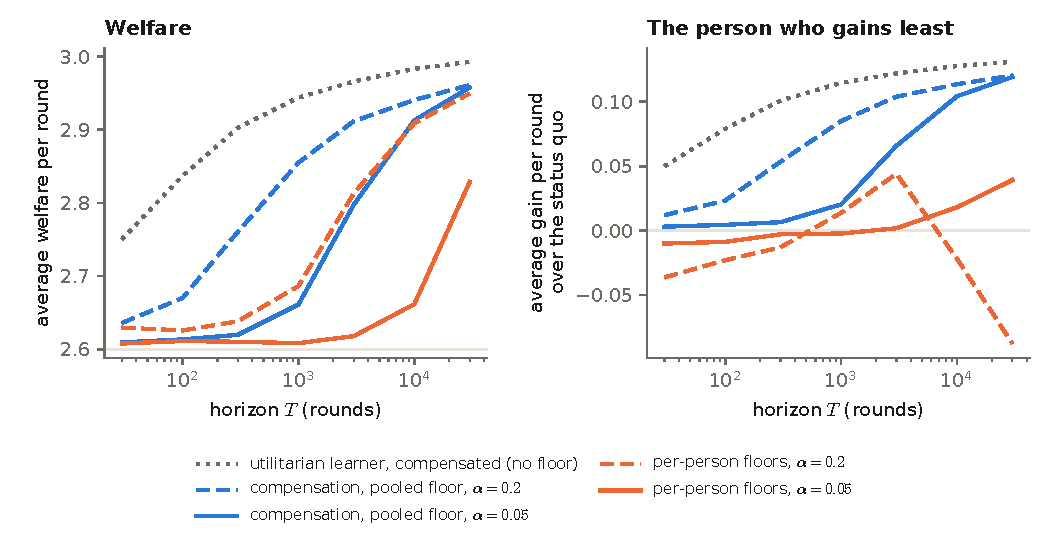
\includegraphics[width=\linewidth]{figures/fig_compare.pdf}
\caption{\Cref{ex:sq}: per-person floors (\cref{sec:sq}) against compensation with a pooled floor and equal shares. Left: welfare per round, averaged over the horizon. Right: the average gain over the status quo of whoever gains least; under compensation everyone gains the same. Means over 40 runs (200 for the utilitarian learner).}
\label{fig:compare}
\end{figure}

\subsection{What each assumes}

Compensation does better on every measure above, and it assumes more.
\begin{itemize}[leftmargin=*,itemsep=1pt]
  \item \emph{A common unit.} Rewards must be transferable one for one. Losses of health, status or liberty are not made good by a payment of equal size, and a person short of money values a payment more than a person who is not.
  \item \emph{Honest, observable outcomes.} The scheme pays each person the gap between their status-quo reward and their realised reward. A person who is fully insured against their own reported outcome has no reason to report it truthfully or to take care over it.
  \item \emph{A known status quo for each person.} The insurance is defined relative to $\mu_{i,a_0}$. Disputes about what someone would have had are disputes about the size of the payment.
  \item \emph{Agreed shares.} The scheme turns a question about policies into a question about dividing a surplus. Equal shares give person 3 in \cref{ex:sq} a gain of $0.13$ where $\astar$ without transfers gives $0.80$.
  \item \emph{Levies.} In a round with a negative surplus the scheme collects from everyone. The floor limits the expected levy, not the realised one.
\end{itemize}
Per-person floors assume none of this. They are what protection costs when people cannot be paid: welfare forgone in every round, and a wait that is set by the person with least to spare.
